\chapter{Ordenamiento}

\index{ordenamiento}

\key{Ordenamiento}
es un problema fundamental en el diseño de algoritmos.
Muchos algoritmos eficientes
usan el ordenamiento como una subrutina,
ya que a menudo es más fácil procesar
datos si los elementos están en orden.

Por ejemplo, el problema "¿un arreglo contiene
dos elementos iguales?" es fácil de resolver usando ordenamiento.
Si el arreglo contiene dos elementos iguales,
estarán uno al lado del otro después de ordenar,
así que es fácil encontrarlos.
Además, el problema "¿cuál es el elemento más frecuente
en un arreglo?" se puede resolver de manera similar.

Hay muchos algoritmos para ordenar, y también son
buenos ejemplos de cómo aplicar
diferentes técnicas de diseño de algoritmos.
Los algoritmos generales de ordenamiento eficientes
funcionan en tiempo $O(n \log n)$,
y muchos algoritmos que utilizan ordenamiento
como una subrutina también
tienen esta complejidad de tiempo.

\section{Teoría del ordenamiento}

El problema básico en el ordenamiento es el siguiente:
\begin{framed}
\noindent
Dado un arreglo que contiene $n$ elementos,
tu tarea es ordenar los elementos
en orden ascendente.
\end{framed}
\noindent
Por ejemplo, el arreglo
\begin{center}
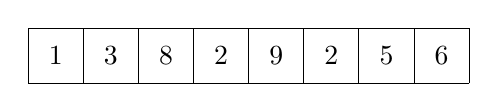
\begin{tikzpicture}[scale=0.7]
\draw (0,0) grid (8,1);
\node at (0.5,0.5) {$1$};
\node at (1.5,0.5) {$3$};
\node at (2.5,0.5) {$8$};
\node at (3.5,0.5) {$2$};
\node at (4.5,0.5) {$9$};
\node at (5.5,0.5) {$2$};
\node at (6.5,0.5) {$5$};
\node at (7.5,0.5) {$6$};
\end{tikzpicture}
\end{center}
será como sigue después de ordenar:
\begin{center}
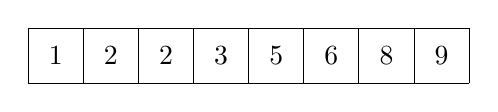
\begin{tikzpicture}[scale=0.7]
\draw (0,0) grid (8,1);
\node at (0.5,0.5) {$1$};
\node at (1.5,0.5) {$2$};
\node at (2.5,0.5) {$2$};
\node at (3.5,0.5) {$3$};
\node at (4.5,0.5) {$5$};
\node at (5.5,0.5) {$6$};
\node at (6.5,0.5) {$8$};
\node at (7.5,0.5) {$9$};
\end{tikzpicture}
\end{center}

\subsubsection{Algoritmos $O(n^2)$}

\index{ordenamiento burbuja}

Los algoritmos simples para ordenar un arreglo
funcionan en tiempo $O(n^2)$.
Estos algoritmos son cortos y generalmente
consisten en dos bucles anidados.
Un famoso algoritmo de ordenamiento en tiempo $O(n^2)$
es el \key{ordenamiento burbuja}, donde los elementos
''burbujean'' en el arreglo según sus valores.

Bubble sort consta de $n$ rondas.
En cada ronda, el algoritmo itera a través
de los elementos del arreglo.
Siempre que se encuentran dos elementos consecutivos
que no están en el orden correcto,
el algoritmo los intercambia.
El algoritmo se puede implementar de la siguiente manera:
\begin{lstlisting}
for (int i = 0; i < n; i++) {
    for (int j = 0; j < n-1; j++) {
        if (array[j] > array[j+1]) {
            swap(array[j],array[j+1]);
        }
    }
}
\end{lstlisting}

Después de la primera ronda del algoritmo,
el elemento más grande estará en la posición correcta,
y en general, después de $k$ rondas, los $k$ elementos más grandes
estarán en las posiciones correctas.
Por lo tanto, después de $n$ rondas, todo el arreglo
estará ordenado.

Por ejemplo, en el arreglo

\begin{center}
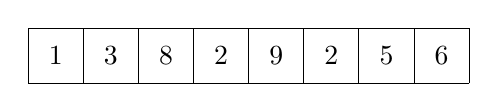
\begin{tikzpicture}[scale=0.7]
\draw (0,0) grid (8,1);

\node at (0.5,0.5) {$1$};
\node at (1.5,0.5) {$3$};
\node at (2.5,0.5) {$8$};
\node at (3.5,0.5) {$2$};
\node at (4.5,0.5) {$9$};
\node at (5.5,0.5) {$2$};
\node at (6.5,0.5) {$5$};
\node at (7.5,0.5) {$6$};
\end{tikzpicture}
\end{center}

\noindent
la primera ronda de bubble sort intercambia elementos
como sigue:

\begin{center}
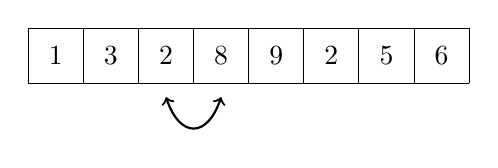
\begin{tikzpicture}[scale=0.7]
\draw (0,0) grid (8,1);
\node at (0.5,0.5) {$1$};
\node at (1.5,0.5) {$3$};
\node at (2.5,0.5) {$2$};
\node at (3.5,0.5) {$8$};
\node at (4.5,0.5) {$9$};
\node at (5.5,0.5) {$2$};
\node at (6.5,0.5) {$5$};
\node at (7.5,0.5) {$6$};

\draw[thick,<->] (3.5,-0.25) .. controls (3.25,-1.00) and (2.75,-1.00) .. (2.5,-0.25);
\end{tikzpicture}
\end{center}

\begin{center}
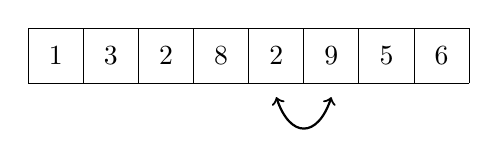
\begin{tikzpicture}[scale=0.7]
\draw (0,0) grid (8,1);
\node at (0.5,0.5) {$1$};
\node at (1.5,0.5) {$3$};
\node at (2.5,0.5) {$2$};
\node at (3.5,0.5) {$8$};
\node at (4.5,0.5) {$2$};
\node at (5.5,0.5) {$9$};
\node at (6.5,0.5) {$5$};
\node at (7.5,0.5) {$6$};

\draw[thick,<->] (5.5,-0.25) .. controls (5.25,-1.00) and (4.75,-1.00) .. (4.5,-0.25);
\end{tikzpicture}
\end{center}

\begin{center}
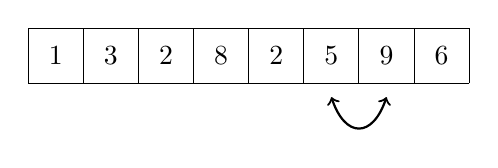
\begin{tikzpicture}[scale=0.7]
\draw (0,0) grid (8,1);
\node at (0.5,0.5) {$1$};
\node at (1.5,0.5) {$3$};
\node at (2.5,0.5) {$2$};
\node at (3.5,0.5) {$8$};
\node at (4.5,0.5) {$2$};
\node at (5.5,0.5) {$5$};
\node at (6.5,0.5) {$9$};
\node at (7.5,0.5) {$6$};

\draw[thick,<->] (6.5,-0.25) .. controls (6.25,-1.00) and (5.75,-1.00) .. (5.5,-0.25);
\end{tikzpicture}
\end{center}

\begin{center}
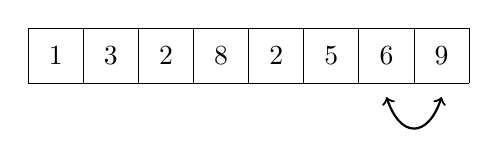
\begin{tikzpicture}[scale=0.7]
\draw (0,0) grid (8,1);
\node at (0.5,0.5) {$1$};
\node at (1.5,0.5) {$3$};
\node at (2.5,0.5) {$2$};
\node at (3.5,0.5) {$8$};
\node at (4.5,0.5) {$2$};
\node at (5.5,0.5) {$5$};
\node at (6.5,0.5) {$6$};
\node at (7.5,0.5) {$9$};

\draw[thick,<->] (7.5,-0.25) .. controls (7.25,-1.00) and (6.75,-1.00) .. (6.5,-0.25);
\end{tikzpicture}
\end{center}

\subsubsection{Inversiones}

\index{inversión}

Bubble sort es un ejemplo de un algoritmo de ordenamiento
que siempre intercambia elementos \emph{consecutivos}
en el arreglo.
Resulta que la complejidad temporal
de tal algoritmo es \emph{siempre}
al menos $O(n^2)$, porque en el peor caso,
se requieren $O(n^2)$ intercambios para ordenar el arreglo.

Un concepto útil al analizar algoritmos de ordenamiento
es una \key{inversión}:
un par de elementos del arreglo
$(\texttt{array}[a],\texttt{array}[b])$ tal que
$a<b$ y $\texttt{array}[a]>\texttt{array}[b]$,
es decir, los elementos están en el orden incorrecto.
Por ejemplo, el arreglo
\begin{center}
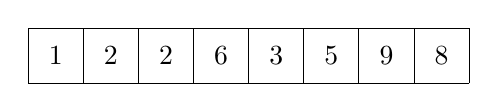
\begin{tikzpicture}[scale=0.7]
\draw (0,0) grid (8,1);
\node at (0.5,0.5) {$1$};
\node at (1.5,0.5) {$2$};
\node at (2.5,0.5) {$2$};
\node at (3.5,0.5) {$6$};
\node at (4.5,0.5) {$3$};
\node at (5.5,0.5) {$5$};
\node at (6.5,0.5) {$9$};
\node at (7.5,0.5) {$8$};
\end{tikzpicture}
\end{center}
tiene tres inversiones: $(6,3)$, $(6,5)$ y $(9,8)$.
El número de inversiones indica
cuánto trabajo se necesita para ordenar el arreglo.
Un arreglo está completamente ordenado cuando
no hay inversiones.
Por otro lado, si los elementos del arreglo
están en orden inverso,
el número de inversiones es el mayor posible:
\[1+2+\cdots+(n-1)=\frac{n(n-1)}{2} = O(n^2)\]

Intercambiar un par de elementos consecutivos que están
en el orden incorrecto elimina exactamente una inversión
del arreglo.
Por lo tanto, si un algoritmo de ordenamiento solo puede
intercambiar elementos consecutivos, cada intercambio elimina
como máximo una inversión, y la complejidad en tiempo
del algoritmo es al menos $O(n^2)$.

\subsubsection{$O(n \log n)$ algoritmos}

\index{ordenamiento por mezcla}

Es posible ordenar un arreglo de manera eficiente
en tiempo $O(n \log n)$ utilizando algoritmos
que no se limitan a intercambiar elementos consecutivos.
Un algoritmo de este tipo es el \key{ordenamiento por mezcla}\footnote{Según \cite{knu983},
el ordenamiento por mezcla fue inventado por J. von Neumann en 1945.},
que se basa en la recursión.

El ordenamiento por mezcla ordena un subarreglo \texttt{array}$[a \ldots b]$ de la siguiente manera:

\begin{enumerate}
\item Si $a=b$, no hacer nada, porque el subarreglo ya está ordenado.
\item Calcular la posición del elemento medio: $k=\lfloor (a+b)/2 \rfloor$.
\item Ordenar recursivamente el subarreglo \texttt{array}$[a \ldots k]$.
\item Ordenar recursivamente el subarreglo \texttt{array}$[k+1 \ldots b]$.
\item \emph{Mezclar} los subarreglos ordenados \texttt{array}$[a \ldots k]$ y
\texttt{array}$[k+1 \ldots b]$
en un subarreglo ordenado \texttt{array}$[a \ldots b]$.
\end{enumerate}

El ordenamiento por mezcla es un algoritmo eficiente, ya que
reduce a la mitad el tamaño del subarreglo en cada paso.
La recursión consta de $O(\log n)$ niveles,
y procesar cada nivel toma $O(n)$ tiempo.
Mezclar los subarreglos \texttt{array}$[a \ldots k]$ y \texttt{array}$[k+1 \ldots b]$
es posible en tiempo lineal, porque ya están ordenados.

Por ejemplo, considere ordenar el siguiente arreglo:
\begin{center}
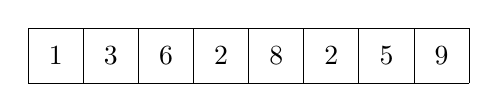
\begin{tikzpicture}[scale=0.7]
\draw (0,0) grid (8,1);
\node at (0.5,0.5) {$1$};
\node at (1.5,0.5) {$3$};
\node at (2.5,0.5) {$6$};
\node at (3.5,0.5) {$2$};
\node at (4.5,0.5) {$8$};
\node at (5.5,0.5) {$2$};
\node at (6.5,0.5) {$5$};
\node at (7.5,0.5) {$9$};
\end{tikzpicture}
\end{center}

El arreglo se dividirá en dos subarreglos
de la siguiente manera:
\begin{center}
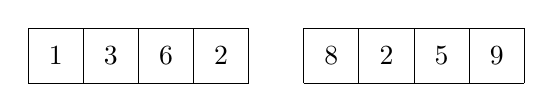
\begin{tikzpicture}[scale=0.7]
\draw (0,0) grid (4,1);
\draw (5,0) grid (9,1);

\node at (0.5,0.5) {$1$};
\node at (1.5,0.5) {$3$};
\node at (2.5,0.5) {$6$};
\node at (3.5,0.5) {$2$};

\node at (5.5,0.5) {$8$};
\node at (6.5,0.5) {$2$};
\node at (7.5,0.5) {$5$};
\node at (8.5,0.5) {$9$};
\end{tikzpicture}
\end{center}

Entonces, los subarreglos se ordenarán recursivamente
de la siguiente manera:
\begin{center}
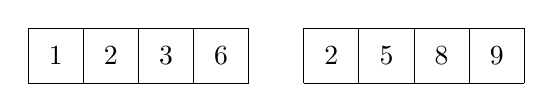
\begin{tikzpicture}[scale=0.7]
\draw (0,0) grid (4,1);
\draw (5,0) grid (9,1);

\node at (0.5,0.5) {$1$};
\node at (1.5,0.5) {$2$};
\node at (2.5,0.5) {$3$};
\node at (3.5,0.5) {$6$};

\node at (5.5,0.5) {$2$};
\node at (6.5,0.5) {$5$};
\node at (7.5,0.5) {$8$};
\node at (8.5,0.5) {$9$};
\end{tikzpicture}
\end{center}

Finalmente, el algoritmo combina los subarreglos ordenados
y crea el arreglo ordenado final:
\begin{center}
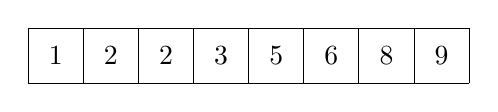
\begin{tikzpicture}[scale=0.7]
\draw (0,0) grid (8,1);
\node at (0.5,0.5) {$1$};
\node at (1.5,0.5) {$2$};
\node at (2.5,0.5) {$2$};
\node at (3.5,0.5) {$3$};
\node at (4.5,0.5) {$5$};
\node at (5.5,0.5) {$6$};
\node at (6.5,0.5) {$8$};
\node at (7.5,0.5) {$9$};
\end{tikzpicture}
\end{center}

\subsubsection{Cota inferior de ordenamiento}

¿Es posible ordenar un arreglo más rápido
que en tiempo $O(n \log n)$?
Resulta que esto \emph{no} es posible
cuando nos limitamos a algoritmos de ordenamiento
que se basan en comparar elementos del arreglo.

La cota inferior para la complejidad del tiempo
se puede demostrar considerando el ordenamiento
como un proceso en el que cada comparación de dos elementos
proporciona más información sobre el contenido del arreglo.
El proceso crea el siguiente árbol:

\begin{center}
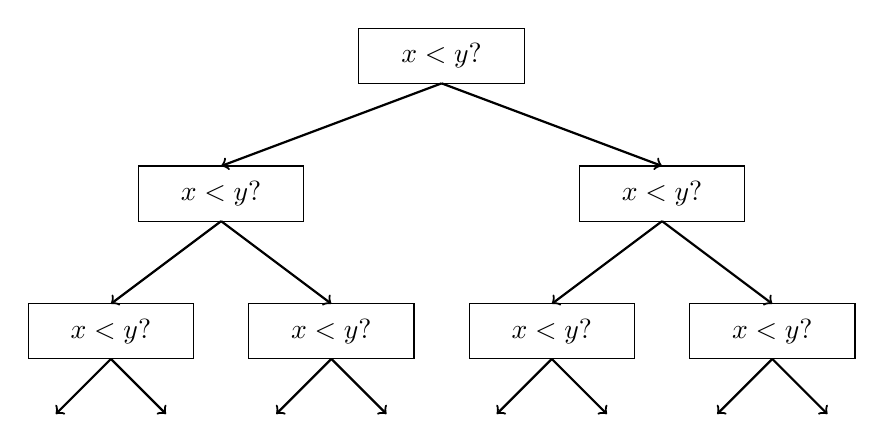
\begin{tikzpicture}[scale=0.7]
\draw (0,0) rectangle (3,1);
\node at (1.5,0.5) {$x < y?$};

\draw[thick,->] (1.5,0) -- (-2.5,-1.5);
\draw[thick,->] (1.5,0) -- (5.5,-1.5);

\draw (-4,-2.5) rectangle (-1,-1.5);
\draw (4,-2.5) rectangle (7,-1.5);
\node at (-2.5,-2) {$x < y?$};
\node at (5.5,-2) {$x < y?$};

\draw[thick,->] (-2.5,-2.5) -- (-4.5,-4);
\draw[thick,->] (-2.5,-2.5) -- (-0.5,-4);
\draw[thick,->] (5.5,-2.5) -- (3.5,-4);
\draw[thick,->] (5.5,-2.5) -- (7.5,-4);

\draw (-6,-5) rectangle (-3,-4);
\draw (-2,-5) rectangle (1,-4);
\draw (2,-5) rectangle (5,-4);
\draw (6,-5) rectangle (9,-4);
\node at (-4.5,-4.5) {$x < y?$};
\node at (-0.5,-4.5) {$x < y?$};
\node at (3.5,-4.5) {$x < y?$};
\node at (7.5,-4.5) {$x < y?$};

\draw[thick,->] (-4.5,-5) -- (-5.5,-6);
\draw[thick,->] (-4.5,-5) -- (-3.5,-6);
\draw[thick,->] (-0.5,-5) -- (0.5,-6);
\draw[thick,->] (-0.5,-5) -- (-1.5,-6);
\draw[thick,->] (3.5,-5) -- (2.5,-6);
\draw[thick,->] (3.5,-5) -- (4.5,-6);
\draw[thick,->] (7.5,-5) -- (6.5,-6);
\draw[thick,->] (7.5,-5) -- (8.5,-6);
\end{tikzpicture}
\end{center}

Aquí ''$x<y?$'' significa que algunos elementos
$x$ y $y$ son comparados.
Si $x<y$, el proceso continúa a la izquierda,
y en caso contrario a la derecha.
Los resultados del proceso son las posibles
maneras de ordenar el arreglo, un total de $n!$ maneras.
Por esta razón, la altura del árbol
debe ser al menos
\[ \log_2(n!) = \log_2(1)+\log_2(2)+\cdots+\log_2(n).\]
Obtenemos una cota inferior para esta suma
al elegir los últimos $n/2$ elementos y
cambiar el valor de cada elemento a $\log_2(n/2)$.
Esto produce una estimación
\[ \log_2(n!) \ge (n/2) \cdot \log_2(n/2),\]
por lo que la altura del árbol y el mínimo
número posible de pasos en un algoritmo de ordenamiento
en el peor caso
es al menos $n \log n$.

\subsubsection{Ordenamiento por conteo}

\index{ordenamiento por conteo}

La cota inferior $n \log n$ no se aplica a
algoritmos que no comparan elementos del arreglo
sino que utilizan alguna otra información.
Un ejemplo de tal algoritmo es
\key{ordenamiento por conteo} que ordena un arreglo en
tiempo $O(n)$ suponiendo que cada elemento en el arreglo
es un entero entre $0 \ldots c$ y $c=O(n)$.

El algoritmo crea un arreglo de \emph{registro},
cuyos índices son elementos del arreglo original.
El algoritmo itera a través del arreglo original
y calcula cuántas veces aparece cada elemento
en el arreglo.
\newpage

Por ejemplo, el arreglo
\begin{center}
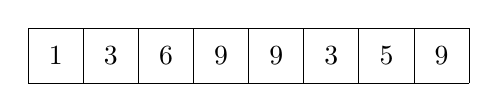
\begin{tikzpicture}[scale=0.7]
\draw (0,0) grid (8,1);
\node at (0.5,0.5) {$1$};
\node at (1.5,0.5) {$3$};
\node at (2.5,0.5) {$6$};
\node at (3.5,0.5) {$9$};
\node at (4.5,0.5) {$9$};
\node at (5.5,0.5) {$3$};
\node at (6.5,0.5) {$5$};
\node at (7.5,0.5) {$9$};
\end{tikzpicture}
\end{center}
corresponde al siguiente arreglo de registro:
\begin{center}
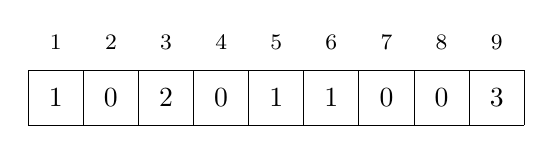
\begin{tikzpicture}[scale=0.7]
\draw (0,0) grid (9,1);
\node at (0.5,0.5) {$1$};
\node at (1.5,0.5) {$0$};
\node at (2.5,0.5) {$2$};
\node at (3.5,0.5) {$0$};
\node at (4.5,0.5) {$1$};
\node at (5.5,0.5) {$1$};
\node at (6.5,0.5) {$0$};
\node at (7.5,0.5) {$0$};
\node at (8.5,0.5) {$3$};

\footnotesize

\node at (0.5,1.5) {$1$};
\node at (1.5,1.5) {$2$};
\node at (2.5,1.5) {$3$};
\node at (3.5,1.5) {$4$};
\node at (4.5,1.5) {$5$};
\node at (5.5,1.5) {$6$};
\node at (6.5,1.5) {$7$};
\node at (7.5,1.5) {$8$};
\node at (8.5,1.5) {$9$};
\end{tikzpicture}
\end{center}

Por ejemplo, el valor en la posición 3
en el arreglo de registro es 2,
porque el elemento 3 aparece 2 veces
en el arreglo original.

La construcción del arreglo de registro
toma un tiempo de $O(n)$. Después de esto, el arreglo ordenado
se puede crear en tiempo $O(n)$ porque
el número de ocurrencias de cada elemento se puede obtener
del arreglo de registro.
Por lo tanto, la complejidad total en tiempo del
ordenamiento por conteo es $O(n)$.

El ordenamiento por conteo es un algoritmo muy eficiente
pero solo se puede usar cuando la constante $c$
es lo suficientemente pequeña, de modo que los elementos del arreglo puedan
usarse como índices en el arreglo de registro.

\section{Ordenamiento en C++}

\index{sort@\texttt{sort}}

Casi nunca es una buena idea usar
un algoritmo de ordenamiento casero
en un concurso, porque hay buenas
implementaciones disponibles en los lenguajes de programación.
Por ejemplo, la biblioteca estándar de C++ contiene
la función \texttt{sort} que se puede utilizar fácilmente para
ordenar arreglos y otras estructuras de datos.

Hay muchos beneficios al usar una función de biblioteca.
En primer lugar, ahorra tiempo porque no hay necesidad de
implementar la función.
En segundo lugar, la implementación de la biblioteca es
ciertamente correcta y eficiente: no es probable
que una función de ordenamiento casera sea mejor.

En esta sección veremos cómo utilizar la
función \texttt{sort} de C++.
El siguiente código ordena
un vector en orden creciente:
\begin{lstlisting}
vector<int> v = {4,2,5,3,5,8,3};
sort(v.begin(),v.end());
\end{lstlisting}
Después del ordenamiento, el contenido del
vector será
$[2,3,3,4,5,5,8]$.
El orden de clasificación predeterminado es creciente,
pero un orden inverso es posible de la siguiente manera:
\begin{lstlisting}
sort(v.rbegin(),v.rend());
\end{lstlisting}
Se puede ordenar un arreglo ordinario de la siguiente manera:
\begin{lstlisting}
int n = 7; // tamaño del arreglo
int a[] = {4,2,5,3,5,8,3};
sort(a,a+n);
\end{lstlisting}
\newpage
El siguiente código ordena la cadena \texttt{s}:
\begin{lstlisting}
string s = "monkey";
sort(s.begin(), s.end());
\end{lstlisting}
Ordenar una cadena significa que los caracteres
de la cadena se ordenan.
Por ejemplo, la cadena ''monkey'' se convierte en ''ekmnoy''.

\subsubsection{Comparison operators}

\index{comparison operator}

The function \texttt{sort} requires that
a \key{comparison operator} is defined for the data type
of the elements to be sorted.
When sorting, this operator will be used
whenever it is necessary to find out the order of two elements.

Most C++ data types have a built-in comparison operator,
and elements of those types can be sorted automatically.
For example, numbers are sorted according to their values
and strings are sorted in alphabetical order.

\index{pair@\texttt{pair}}

Pairs (\texttt{pair}) are sorted primarily according to their
first elements (\texttt{first}).
However, if the first elements of two pairs are equal,
they are sorted according to their second elements (\texttt{second}):
\begin{lstlisting}
vector<pair<int,int>> v;
v.push_back({1,5});
v.push_back({2,3});
v.push_back({1,2});
sort(v.begin(), v.end());
\end{lstlisting}
After this, the order of the pairs is
$(1,2)$, $(1,5)$ and $(2,3)$.

\index{tuple@\texttt{tuple}}

In a similar way, tuples (\texttt{tuple})
are sorted primarily by the first element,
secondarily by the second element, etc.\footnote{Note that in some older compilers,
the function \texttt{make\_tuple} has to be used to create a tuple instead of
braces (for example, \texttt{make\_tuple(2,1,4)} instead of \texttt{\{2,1,4\}}).}:
\begin{lstlisting}
vector<tuple<int,int,int>> v;
v.push_back({2,1,4});
v.push_back({1,5,3});
v.push_back({2,1,3});
sort(v.begin(), v.end());
\end{lstlisting}
After this, the order of the tuples is
$(1,5,3)$, $(2,1,3)$ and $(2,1,4)$.

\subsubsection{User-defined structs}

User-defined structs do not have a comparison
operator automatically.
The operator should be defined inside
the struct as a function
\texttt{operator<},
whose parameter is another element of the same type.
The operator should return \texttt{true}
if the element is smaller than the parameter,
and \texttt{false} otherwise.

For example, the following struct \texttt{P}
contains the x and y coordinates of a point.
The comparison operator is defined so that
the points are sorted primarily by the x coordinate
and secondarily by the y coordinate.

\begin{lstlisting}
struct P {
    int x, y;
    bool operator<(const P &p) {
        if (x != p.x) return x < p.x;
        else return y < p.y;
    }
};
\end{lstlisting}

\subsubsection{Comparison functions}

\index{comparison function}

It is also possible to give an external
\key{comparison function} to the \texttt{sort} function
as a callback function.
For example, the following comparison function \texttt{comp}
sorts strings primarily by length and secondarily
by alphabetical order:

\begin{lstlisting}
bool comp(string a, string b) {
    if (a.size() != b.size()) return a.size() < b.size();
    return a < b;
}
\end{lstlisting}
Now a vector of strings can be sorted as follows:
\begin{lstlisting}
sort(v.begin(), v.end(), comp);
\end{lstlisting}

\section{Binary search}

\index{binary search}

A general method for searching for an element
in an array is to use a \texttt{for} loop
that iterates through the elements of the array.
For example, the following code searches for
an element $x$ in an array:

\begin{lstlisting}
for (int i = 0; i < n; i++) {
    if (array[i] == x) {
        // x found at index i
    }
}
\end{lstlisting}

The time complexity of this approach is $O(n)$,
because in the worst case, it is necessary to check
all elements of the array.
If the order of the elements is arbitrary,
this is also the best possible approach, because
there is no additional information available where
in the array we should search for the element $x$.

However, if the array is \emph{sorted},
the situation is different.
In this case it is possible to perform the
search much faster, because the order of the
elements in the array guides the search.
The following \key{binary search} algorithm
efficiently searches for an element in a sorted array
in $O(\log n)$ time.

\subsubsection{Method 1}

The usual way to implement binary search
resembles looking for a word in a dictionary.
The search maintains an active region in the array,
which initially contains all array elements.
Then, a number of steps is performed,
each of which halves the size of the region.

At each step, the search checks the middle element
of the active region.
If the middle element is the target element,
the search terminates.
Otherwise, the search recursively continues
to the left or right half of the region,
depending on the value of the middle element.

The above idea can be implemented as follows:
\begin{lstlisting}
int a = 0, b = n-1;
while (a <= b) {
    int k = (a+b)/2;
    if (array[k] == x) {
        // x found at index k
    }
    if (array[k] > x) b = k-1;
    else a = k+1;
}
\end{lstlisting}

In this implementation, the active region is $a \ldots b$,
and initially the region is $0 \ldots n-1$.
The algorithm halves the size of the region at each step,
so the time complexity is $O(\log n)$.

\subsubsection{Method 2}

An alternative method to implement binary search
is based on an efficient way to iterate through
the elements of the array.
The idea is to make jumps and slow the speed
when we get closer to the target element.

The search goes through the array from left to
right, and the initial jump length is $n/2$.
At each step, the jump length will be halved:
first $n/4$, then $n/8$, $n/16$, etc., until
finally the length is 1.
After the jumps, either the target element has
been found or we know that it does not appear in the array.

The following code implements the above idea:
\begin{lstlisting}
int k = 0;
for (int b = n/2; b >= 1; b /= 2) {
    while (k+b < n && array[k+b] <= x) k += b;
}
if (array[k] == x) {
    // x found at index k
}
\end{lstlisting}

During the search, the variable $b$
contains the current jump length.
The time complexity of the algorithm is $O(\log n)$,
because the code in the \texttt{while} loop
is performed at most twice for each jump length.

\subsubsection{C++ functions}

The C++ standard library contains the following functions
that are based on binary search and work in logarithmic time:

\begin{itemize}
\item \texttt{lower\_bound} returns a pointer to the
first array element whose value is at least $x$.
\item \texttt{upper\_bound} returns a pointer to the
first array element whose value is larger than $x$.
\item \texttt{equal\_range} returns both above pointers.
\end{itemize}

The functions assume that the array is sorted.
If there is no such element, the pointer points to
the element after the last array element.
For example, the following code finds out whether
an array contains an element with value $x$:

\begin{lstlisting}
auto k = lower_bound(array,array+n,x)-array;
if (k < n && array[k] == x) {
    // x found at index k
}
\end{lstlisting}

Then, the following code counts the number of elements
whose value is $x$:

\begin{lstlisting}
auto a = lower_bound(array, array+n, x);
auto b = upper_bound(array, array+n, x);
cout << b-a << "\n";
\end{lstlisting}

Using \texttt{equal\_range}, the code becomes shorter:

\begin{lstlisting}
auto r = equal_range(array, array+n, x);
cout << r.second-r.first << "\n";
\end{lstlisting}

\subsubsection{Finding the smallest solution}

An important use for binary search is
to find the position where the value of a \emph{function} changes.
Suppose that we wish to find the smallest value $k$
that is a valid solution for a problem.
We are given a function $\texttt{ok}(x)$
that returns \texttt{true} if $x$ is a valid solution
and \texttt{false} otherwise.
In addition, we know that $\texttt{ok}(x)$ is \texttt{false}
when $x<k$ and \texttt{true} when $x \ge k$.
The situation looks as follows:

\begin{center}
\begin{tabular}{r|rrrrrrrr}
$x$ & 0 & 1 & $\cdots$ & $k-1$ & $k$ & $k+1$ & $\cdots$ \\
\hline
$\texttt{ok}(x)$ & \texttt{false} & \texttt{false}
& $\cdots$ & \texttt{false} & \texttt{true} & \texttt{true} & $\cdots$ \\
\end{tabular}
\end{center}

\noindent
Now, the value of $k$ can be found using binary search:

\begin{lstlisting}
int x = -1;
for (int b = z; b >= 1; b /= 2) {
    while (!ok(x+b)) x += b;
}
int k = x+1;
\end{lstlisting}

The search finds the largest value of $x$ for which
$\texttt{ok}(x)$ is \texttt{false}.
Thus, the next value $k=x+1$
is the smallest possible value for which
$\texttt{ok}(k)$ is \texttt{true}.
The initial jump length $z$ has to be
large enough, for example some value
for which we know beforehand that $\texttt{ok}(z)$ is \texttt{true}.

The algorithm calls the function \texttt{ok}
$O(\log z)$ times, so the total time complexity
depends on the function \texttt{ok}.
For example, if the function works in $O(n)$ time,
the total time complexity is $O(n \log z)$.

\subsubsection{Finding the maximum value}

Binary search can also be used to find
the maximum value for a function that is
first increasing and then decreasing.
Our task is to find a position $k$ such that

\begin{itemize}
\item
$f(x)<f(x+1)$ when $x<k$, and
\item
$f(x)>f(x+1)$ when $x \ge k$.
\end{itemize}

The idea is to use binary search
for finding the largest value of $x$
for which $f(x)<f(x+1)$.
This implies that $k=x+1$
because $f(x+1)>f(x+2)$.
The following code implements the search: 

\begin{lstlisting}
int x = -1;
for (int b = z; b >= 1; b /= 2) {
    while (f(x+b) < f(x+b+1)) x += b;
}
int k = x+1;
\end{lstlisting}

Note that unlike in the ordinary binary search,
here it is not allowed that consecutive values
of the function are equal.
In this case it would not be possible to know
how to continue the search.
